\section{Magnetic Field Design}

As described in section \ref{chap:Hall Thruster Theory}, the radial magnetic field in a \ac{HET} traps electrons in an azimuthal Hall current, which allows for a strong axial electric field to be established. The methods of generating this magnetic field considered were:

\begin{itemize}
    \item Electromagnetic Coils
    \item Radial Permanent Magnets
    \item Field shaping with a ferromagnetic core and permanent magnets
\end{itemize}

\subsection{Electromagnetic Coils}

Electromagnetic coils are the most common method of generating the magnetic field as seen in fig \ref{fig:annular_HET}. They allow for the magnetic field strength to be adjusted bu changing the current flowing through the coils. However, they require a significant amount of power to operate, which is not ideal for smaller, lower power thrusters. Additionally, they generated heat which increases the design complexity as further thermal management will be required.

\subsection{Radially Aligned Permanent Magnets}

Another solution is to use ring shaped permanent magnets, placed near the exit plane of the thruster to generate the radial magnetic field as seen in fig \ref{fig:radial-permanent-magnet-concept}. This method does not require any power to operate, and does not generate heat. However, the magnetic field strength cannot be adjusted without physically changing the magnets. Additionally, the custom radially aligned magnets can be expensive to purchase or manufacture.

\subsection{Field Shaping with a Ferromagnetic Core and Permanent Magnets}
The final method considered was to use a ferromagnetic core to shape the magnetic field generated by a set of smaller permanent magnets. This means that a material with high magnetic permeability is used to direct the magnetic field lines from the magnets embedded in the core to the desired locations in the thruster channel. An example of this method can be seen in fig~\ref{fig:ugrad-het-magnetic-shunt}. This method does not require any power to operate, and does not generate heat. Similar to the permanent magnet design proposed above, the magnetic field strength cannot be adjusted without physically changing the magnets. This method also allows for the use of smaller, more common magnets which are cheaper and easier to source.

\begin{figure}[H]
    \centering
    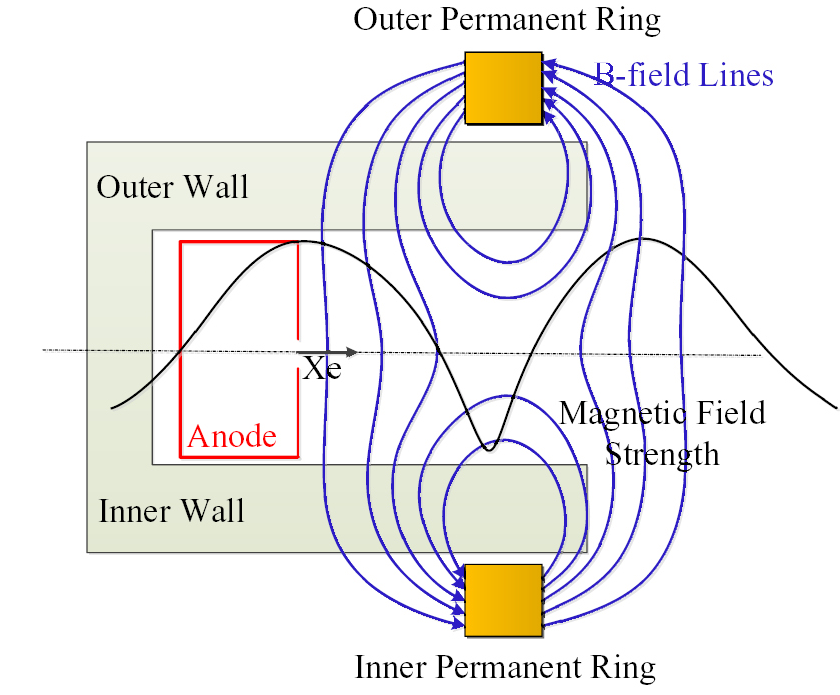
\includegraphics[width=0.5\textwidth]{images/Concepts/radial permanent magnets.png}
    \captionsetup{justification=centering}
    \caption{Magnetic Field concept using radially aligned permanent magnets near the thruster exit plane \cite{Ding_2017}}
    \label{fig:radial-permanent-magnet-concept}
\end{figure}

\begin{figure}[H]
    \centering
    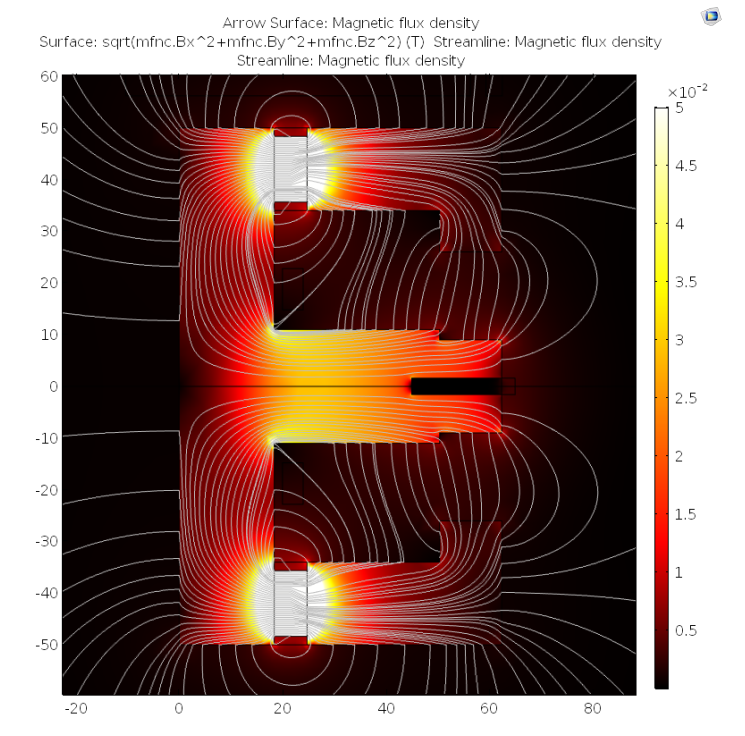
\includegraphics[width=0.7\textwidth]{images/Concepts/UGRAD magnetic shunt.png}
    \captionsetup{justification=centering}
    \caption{Predicted magnetic field lines using a ferromagnetic core and permanent magnets (seen in bright yellow/white) \cite{ugrad-het-olin-college}}
    \label{fig:ugrad-het-magnetic-shunt}
\end{figure}